\section{System setup}

\subsection{Hardware and communication setup}
The host computer controls the entire system.

- The host computer handles the communication to the Pico through serial communication over USB. The Pico controls whether the gripper should open or close.

- A camera is used to detect moves. It communicates with the computer via USB. 

- For control of the robot, the host computer communicates over RTDE.

The overall communication can be seen in.\cref{fig: commdiagram}.

\begin{figure} [H]
    \centering
    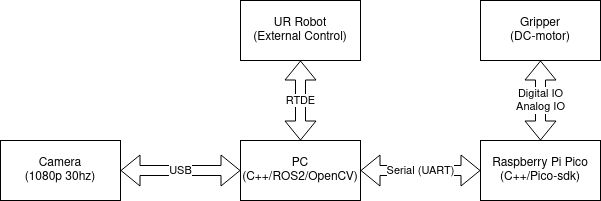
\includegraphics[width=0.7\linewidth]{Pictures/Commdiagram.png}
    \caption{Communication diagram of the various devices used.}
    \label{fig: commdiagram}
\end{figure}

\subsection{Workbench setup} \label{sec: Workbench setup}


\begin{figure} [t]
    \centering
    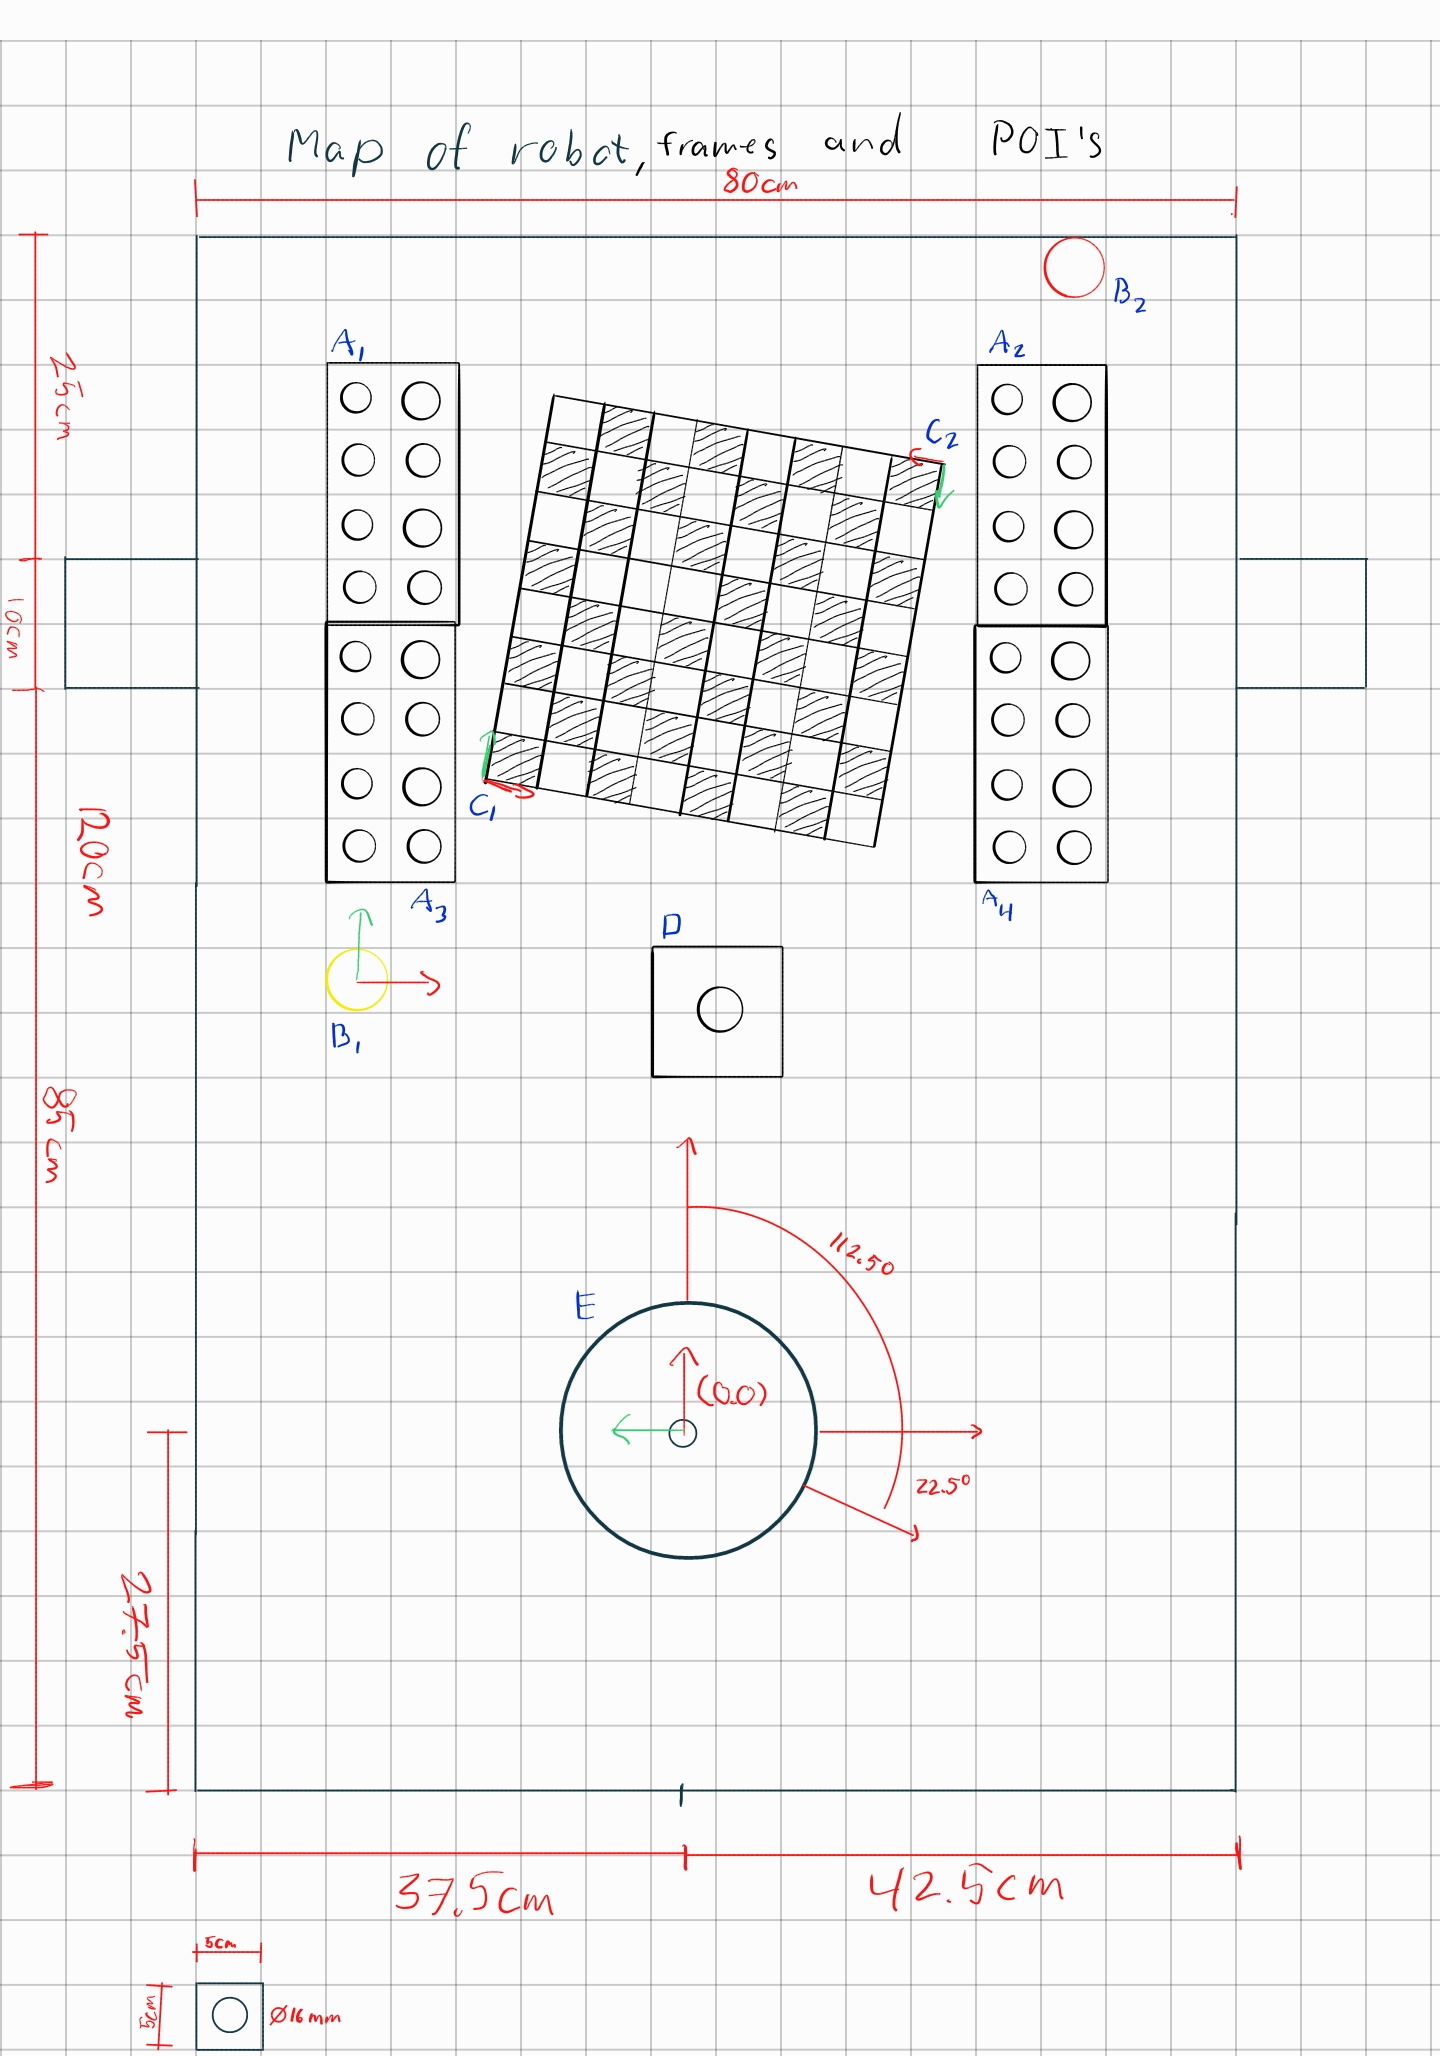
\includegraphics[width=0.7\linewidth]{Pictures/map_of_robot.jpg}
    \caption{Workbench setup. The following markings can be seen: $A$: 4 death position boards. $B$: The yellow and red peg, $C$: The chessboard. $D$: the temporary storage board. $E$: The robot base. $B_1$ \& $C_1$: The two frames used for motionplanning to pieces onboard the chessboard.}
    \label{fig: workbench setup}
\end{figure}

Multiple parts are needed to interact with the robot.

- 4 boards, each with 8 death positions for the pieces.

- An additional board with one position for temporary storage when the player captures.

- A yellow and a red peg meant for configuring the camera and setting up transformation matrices. the position of the yellow peg is used to define said transformation matrix

- The chessboard, which can be placed dynamically between the 4 deathposition plates. The corners of this board must be colored red and green for the purpose of finding it. The green corner will have to be closest to H8 and is used to define the transformation matrix for the chessboard frame.

- The UR-Robot, which is rotated by 112.5\degree \space this is fixed and must be accounted for.

The placement of the parts can be seen on \cref{fig: workbench setup}

\begin{figure} [H]
    \centering
    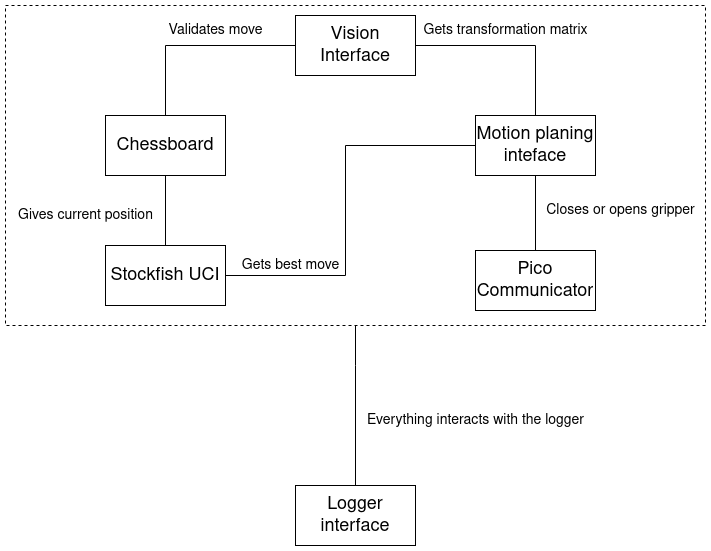
\includegraphics[width=0.7\linewidth]{Pictures/DomainModel.drawio.png}
    \caption{Domain model of the software setup.}
    \label{fig: DomainModel}
\end{figure}
\subsection{Software setup}
As seen on the sequence diagram in \cref{fig: sequencediagram} the program runs sequentially, handling different tasks in order. While comprised of many classes, the program is encapsulated into five different interfaces, each of which is called from a central program running the main code. A simplified domain model of the system can be seen on \cref{fig: DomainModel}.

- The logger interface is initiated before anything relevant to the game starts. It records everything for testing and debugging.

- The motion planning interface handles motion planning and communicates with the robot.

- The vision interface handles image capturing and processing for finding the chessboard and piece movement from players.

- The board interface validates the moves, keeps track of the position of the pieces and interacts with the chess engine.

- The Pico communication interface handles communication with the microcontroller, controlling the gripper.

The Pico runs its own separate program, which primarily listens for commands sent by the main program for opening and closing the gripper.



